\documentclass[refman]{scrartcl}

\usepackage[utf8]{inputenc}

\usepackage[english]{babel}
\usepackage{tikz}
\usepackage{endnotes}
\usetikzlibrary{shapes.geometric, arrows}
\tikzstyle{startstop} = [rectangle, rounded corners, minimum width=3cm, minimum height=1cm,text centered, draw=black, fill=red!30]
\tikzstyle{io} = [trapezium, trapezium left angle=70, trapezium right angle=110, minimum width=3cm, minimum height=1cm, text centered, draw=black, fill=blue!30]
\tikzstyle{process} = [rectangle, minimum width=3cm, minimum height=1cm, text centered, draw=black, fill=orange!30]
\tikzstyle{decision} = [diamond, minimum width=3cm, minimum height=1cm, text centered, draw=black, fill=green!30]
\tikzstyle{arrow} = [thick,->,>=stealth]

\usepackage{fancyhdr}
\usepackage{epigraph}



\usepackage{amsmath}

\usepackage{listings}

\pagestyle{fancy}

\lstdefinestyle{mystyle}{
    backgroundcolor=\color{white},   
    commentstyle=\color{codegreen},
    keywordstyle=\color{Fuchsia},
    numberstyle=\tiny\color{gray},
    stringstyle=\color{codepurple},
    basicstyle=\footnotesize,
    breakatwhitespace=false,         
    breaklines=true,                 
    captionpos=b,                    
    keepspaces=true,                 
    numbers=left,                    
    numbersep=5pt,                  
    showspaces=false,                
    showstringspaces=false,
    showtabs=false,                  
    tabsize=2
}
 
\lstset{style=mystyle}


\newcommand{\mymod}{\text{\ \ mod\ \ }}


\begin{document}

% ----------------------------------------------------------------------------------------------------------
% PREAMBLE
% ----------------------------------------------------------------------------------------------------------

\begin{titlepage}
	\centering
	
\includegraphics[width=0.15\textwidth]{graphics/huberlin_logo}\par\vspace{1cm}
	{\scshape\LARGE Humboldt University of Berlin \par}
	\vspace{1cm}
	{\scshape\Large Einf{\"u}hrung in das wissenschaftliche Rechnen \par}
	\vspace{1.5cm}
	{\huge\bfseries Documentation of Fraction Application Programming Interface and Command Line Interface Calculator\par}
	\vspace{2cm}
	{\Large\itshape Robert A. Bedard \par}
	\vfill

	\vfill

% Bottom of the page
	{\large \today\par}
\end{titlepage}

\tableofcontents
\newpage

\section{User Manual}
Name of the program: bruch

\noindent This program allows the user to enter fractions and reduce and add them.

\noindent The module tools3.py is required.

\noindent After starting it, the user must simply follow the instructions.
\section{Documentation}

\subsection{tools3.py}

In this module, we have the two functions to compute the greatest common divisor and the least common multiple. Here, there are no classes, just free functions.

\begin{itemize}
    \item \texttt{ggt(arg1, arg2)}
    computes the greatest common divisor via Euclidean algorithm.
    \begin{itemize}
        \item Arguments
        \begin{enumerate}
            \item \texttt{arg1} (int): first integer
            \item \texttt{arg2} (int): second integer
        \end{enumerate}
        \item Returns (int): greatest common divisor of the first and second integer
    \end{itemize}
    \item \texttt{kgv(arg1,arg2)}
    determines the least common multiple, utilizing the greatest common divisor, computed by the function \texttt{ggt(arg1, arg2)}.
    \begin{itemize}
        \item Arguments
        \begin{enumerate}
            \item \texttt{arg1} (int): first integer
            \item \texttt{arg2} (int): second integer
        \end{enumerate}
        \item Returns (int): least common multiple of the first and second integer.
    \end{itemize}
    \item \texttt{main()} for testing purposes. Takes no arguments and returns none.
\end{itemize}

\subsection{bruch.py}

In this module, we have implemented the class Bruch that represents fractions.

\subsubsection{class Bruch()}

The objects of this class represent fractions.

\noindent\textbf{Attributes}

\begin{itemize}
    \item zaehler (int): the numerator
    \item nenner (int): the denominator
\end{itemize}

\noindent\textbf{Methodes}

\begin{itemize}
    \item \texttt{kuerzen(self)} reduces the fraction. Takes no arguments except for self and returns none.
    \item \texttt{\_\_add\_\_(self, other)} adds two fractions together via finding the greatest common divisor and reduces afterwards. The result is a new Bruch object.
    \begin{itemize}
        \item Arguments
        \begin{enumerate}
            \item other (Bruch): another fraction
        \end{enumerate}
        \item Returns (Bruch): the sum of the two fractions
    \end{itemize}
    \item \texttt{\_\_repr\_\_(self)} returns a printable string.
    \begin{itemize}
        \item Arguments: none except for self
        \item Returns (str): printable string
    \end{itemize}
    \item \texttt{check\_validity(self)} checks the fraction for validity. Returns false if the denominator is \(0\).
    \begin{itemize}
        \item Arguments: none except for self
        \item Returns (boolean): false if the denominator is \(0\), in any other case true
    \end{itemize}
\end{itemize}

\subsubsection{Free Functions}

\begin{itemize}
    \item \texttt{addiere(bruch\_1, bruch\_2)} adds two fractions into a new fractions
    \begin{itemize}
        \item Arguments
        \begin{enumerate}
            \item \texttt{bruch\_1} (Bruch): first summand
            \item \texttt{bruch\_2} (Bruch): second summand
        \end{enumerate}
        \item Returns (Bruch): the sum of the two fractions
    \end{itemize}
\end{itemize}

\section{Euclidean Algorithm}
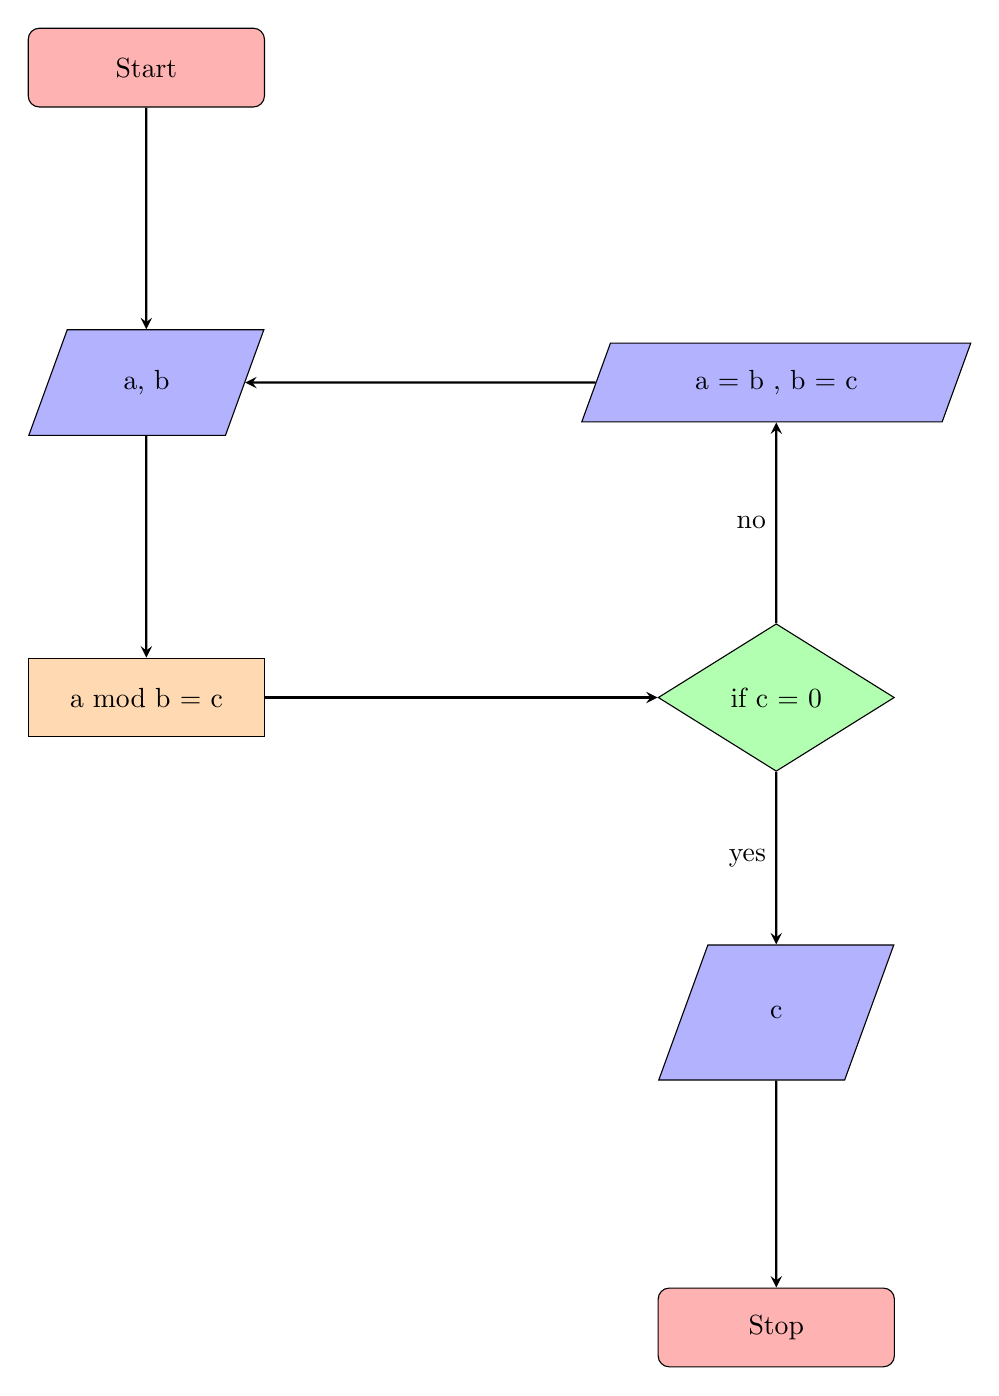
\begin{tikzpicture}[node distance=4cm]
    \node (start) [startstop] {Start};
    \node (in1) [io, below of=start] {a, b};
    \node (pro1) [process, below of=in1] {a mod b = c};
    \node (dec1) [decision, right of=pro1, xshift=4cm] {if c = 0};
    \node (out1) [io, below of=dec1] {c};
    \node (out2) [io, above of=dec1] {a = b , b = c};
    \node (stop) [startstop, below of=out1] {Stop};
    \draw [arrow] (start) -- (in1);
    \draw [arrow] (in1) -- (pro1);
    \draw [arrow] (pro1) -- (dec1);
    \draw [arrow] (dec1) -- node[anchor=east] {no}(out2);
    \draw [arrow] (out2) -- (in1);
    \draw [arrow] (dec1) -- node[anchor=east] {yes}(out1);
    \draw [arrow] (out1) -- (stop);
\end{tikzpicture}
    

\begin{thebibliography}{9}
	\bibitem{Rabus} 
	Rabus, Helga. 
	\textit{EWR Vorlesung}. 
	Humboldt-Universität zu Berlin, 2022.
	
\end{thebibliography}

\end{document}
